\chapter{Architecture and Design}

\section{Scenario Definition and Goal}
\label{sec:scenario_definition}
This project is considering a very specific scenario that involves the transportation of artwork from one place to another. More specifically a \textit{sender} is handing custody of the artwork to a \textit{carrier} who is responsible to transport the artwork safely to a \textit{recipient}. Upon arrival, the artwork's custody is transferred to the \textit{recipient}. During the transportation of the artwork environmental data like temperature and humidity is recorded and made available for monitoring purposes.

\begin{figure}[ht]
    \centering
    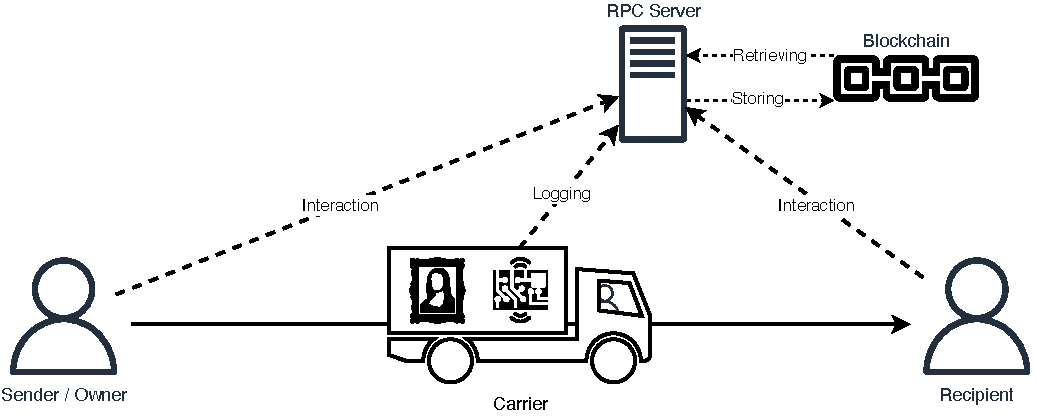
\includegraphics[width=0.8\textwidth]{diagrams/Scenario.drawio.pdf}
    \caption{Defined scenario for the system to consider}
    \label{fig:scenario}
\end{figure}

\subsection*{Goal}
The goal is to create a minimal working system for artwork tracking, considering the following abstractions and the defined scenario. The system should allow the creation of an \gls{nft} associated with a piece of artwork as well as the storing, and retrieval of data on the \gls{nft}.

\subsection*{Summary of Abstractions}
The real-world scenario of transferring custody of artwork for transportation is naturally much more complex and involves more actors \cite{artintransit}. However, in this work we are making the following abstractions:
\begin{itemize}
    \item The sender of a specific artwork is also the owner of the artwork
    \item When considering the transportation of the artwork back to the location of origin, the \textit{sender} and \textit{recipient} are the same.
    \item The authenticity and integrity of the artwork can be verified by any of the actors
\end{itemize}



\section{Overview}
Since the system is considering a very specific scenario This chapter aims to provide a high-level overview of the architecture of the system while later going into detail about its components and actors.

\begin{figure}[ht]
    \centering
    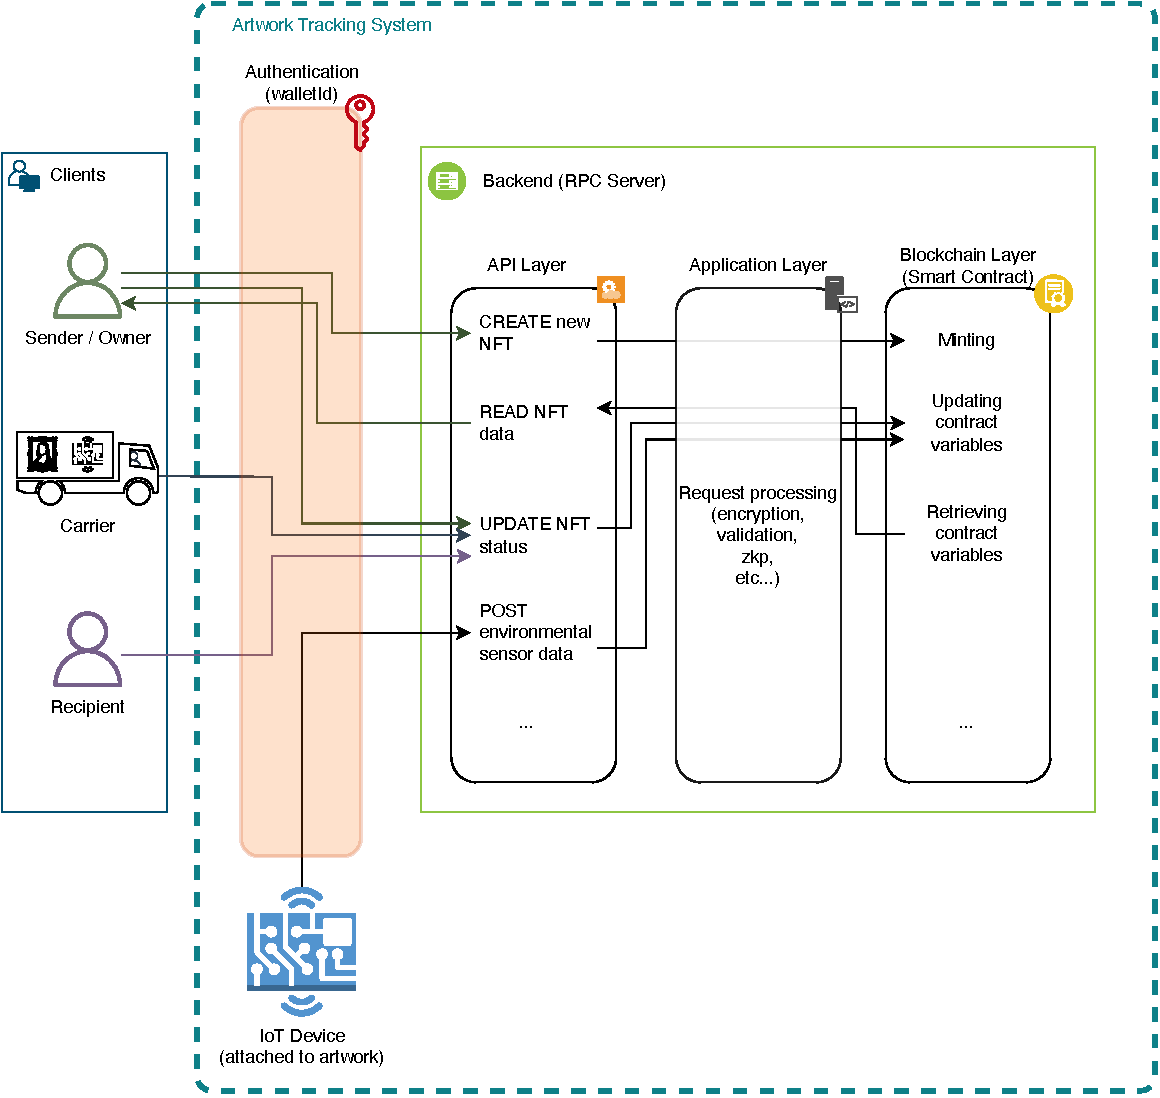
\includegraphics[height=0.5\textheight, keepaspectratio]{diagrams/Architecture.drawio.pdf}
    \caption{High-Level architecture design}
    \label{fig:architecture}
\end{figure}

\subsection{Actors}
As already introduced in the section \nameref{sec:scenario_definition}, the system is designed for three actors. These actors are defined as follows.

\begin{itemize}[align=left, font=\itshape]
    \item[Sender:] A person or institution that is in charge of dispatching the artwork from a departure location to a destination. This Actor is also considered the \textit{owner} of the artwork. In this context, they can be used interchangeably. The responsibilities of this actor include the initial registration of the artwork as an \gls{nft}, the holding of the \gls{nft} in a \gls{wallet}, and the setup of the \gls{iot} device.

    \item[Carrier:] A transportation company responsible for the safe transport of artwork from one location to another. The \textit{carrier} is committed to delivering the artwork without any damage or alteration. They are also responsible to verify the authenticity and integrity together with the \textit{sender} or \textit{recipient} upon departure and arrival respectively.

    \item[Recipient:] A person or institution that is receiving the artwork. They share the responsibilities of the \textit{carrier} to verify the authenticity and integrity of the artwork upon arrival. 
\end{itemize}


\subsection{Technical Components}
Apart from the specified external actors of the system, there are also internal components to consider.

\begin{itemize}[align=left,font=\itshape]
    \item[Logger:] \gls{iot} Device responsible for recording environmental data while the artwork is in transit.  
    % TODO: descirbe which hardware components are involved
    \item[Blockchain:] Decentralized, distributed ledger that stores transactions or data in a secure, tamper-resistant, and tamper-evident fashion. The blockchain can be used to create and track \glspl{nft}, their ownership and provenance as well as the data
    \item[Smart Contract:]  
    \item[Backend (\gls{rpc} Server):]
\end{itemize}

